%!TEX root = ../thesis.tex
%*******************************************************************************
%****************************** Third Chapter **********************************
%*******************************************************************************
\chapter{Evaluation}

% **************************** Define Graphics Path **************************
\ifpdf
    \graphicspath{{Chapter6/Figs/Raster/}{Chapter6/Figs/PDF/}{Chapter6/Figs/}}
\else
    \graphicspath{{Chapter6/Figs/Vector/}{Chapter6/Figs/}}
\fi

\section{Evaluation Settings}

Appendix A presents a list of synthetic functions and real datasets that are used to evaluate the effectiveness of a bayesian optimization algorithm. 
We will briefly go over some synthetic functions that we will be using for the evaluation of our algorithm.
Furthermore, we will shortly discuss the underlying real dataset, which is hyper-parameter-configurations from the SwissFEL x-ray laser.

\section{Quantitative evaluation}

We will conduct experiments in the following settings (as mentioned in some other chapter REEEE):

\begin{enumerate}
\item a 2D embedded function in a 3D (synthetic).
\item a 2D embedded function in a 10D (synthetic).
\item a 5D embedded function in a 25D setting (synthetic).
\item A function that has the exact same structure that we propose.
\item SwissFEL data (5D real dimensional domain).
\end{enumerate}

\section{Qualitative evaluation}

\subsection{Finding a matrix when we apply a polynomial kernel onto the input first}
We want to analyse if the gpregression can identify the random matrix, if the input is first put through a polynomial kernel of degree 2. \\

More specifically, the problem looks as follows.
We want to approximate the real function $ f $ through a gaussian process $ g $, with the following condition:

\def\B{
\begin{bmatrix}
    (x - x_0)^2 \\
    (x - x_1)^2
\end{bmatrix}}

\begin{equation}
f \left( W \B \right) \approx g \left( x \right)
\end{equation} 

where $x_0, x_1$ are constants.


\subsection{Subspace identification}
One of the main reasons to use our method is because we allow for subspace identification.
We have the following functions:

\begin{enumerate}
\item 1D Parabola embedded in a 2D space
\item 2D Camelback embedded in a 5D space
\item 2D Sinusoidal and Exponential function embedded in a 5D space
\item 5D Rosenbrock function embedded in a 10D space
\end{enumerate}

In the following figure, any blue point shows the real function value.
Any orange point shows the point that the mean prediction of the Gaussian Process predicted.
The function was learned using 100 datapoints. 
The points shown below were not used for training at any point.
The predominantly orange figures are respective surrogate functions of this real function.
For each of the methods, the embedding is learned using the respective algorithm.

\newpage
% PARABOLA FUNCTION
\begin{figure}[H]
    \centering
    \begin{subfigure}[b]{0.30\textwidth}
        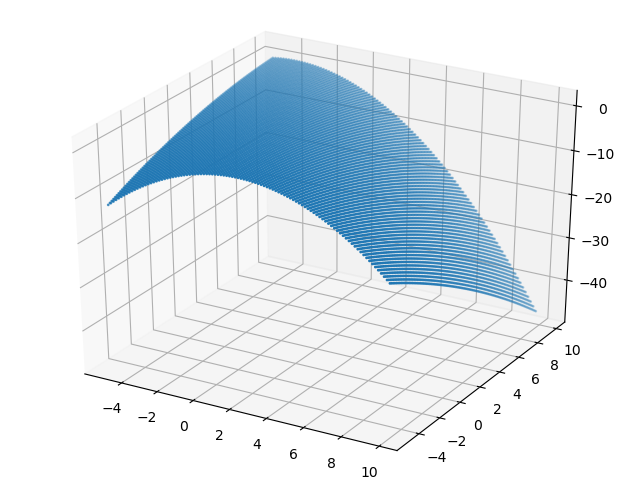
\includegraphics[width=\textwidth]{orig/embedded_parabola_2d_to_1d.png}
        \caption{Parabola Original}
        \label{fig:gull}
    \end{subfigure}
    %add desired spacing between images, e. g. ~, \quad, \qquad, \hfill etc. 
      %(or a blank line to force the subfigure onto a new line)
    \begin{subfigure}[b]{0.30\textwidth}
        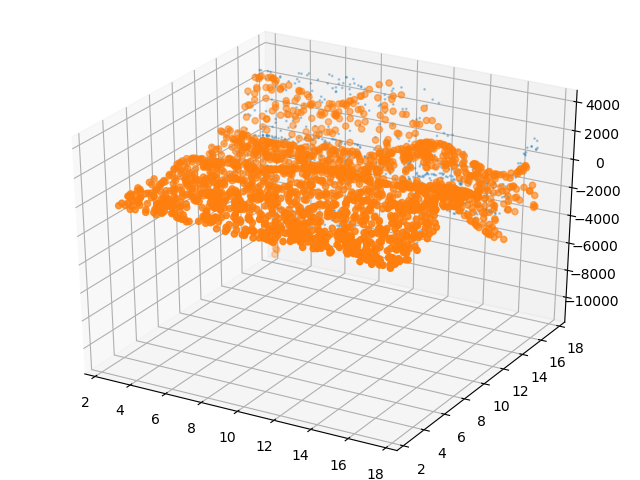
\includegraphics[width=\textwidth]{embedded_sinusoidal_small_perturbations_5d_to_2d_boring.png}
        \caption{Parabolanusoidal Boring}
        \label{fig:tiger}
    \end{subfigure}
     %add desired spacing between images, e. g. ~, \quad, \qquad, \hfill etc. 
    %(or a blank line to force the subfigure onto a new line)
    \vskip\baselineskip
    \begin{subfigure}[b]{0.30\textwidth}
        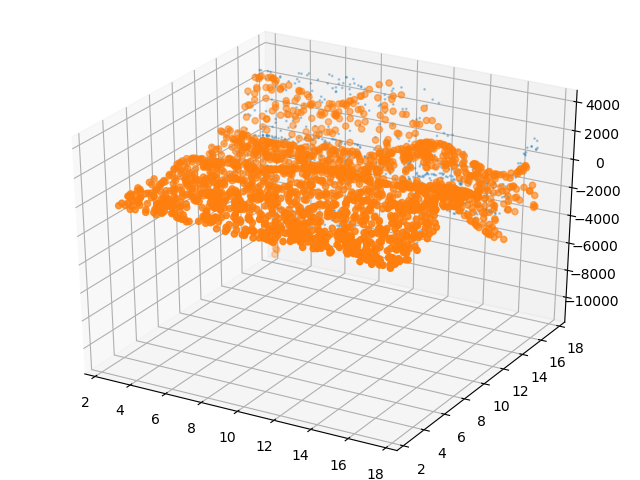
\includegraphics[width=\textwidth]{embedded_sinusoidal_small_perturbations_5d_to_2d_boring.png}
        \caption{Parabola Tripathy}
        \label{fig:mouse}
    \end{subfigure}
            %add desired spacing between images, e. g. ~, \quad, \qquad, \hfill etc. 
    %(or a blank line to force the subfigure onto a new line)
    \begin{subfigure}[b]{0.30\textwidth}
        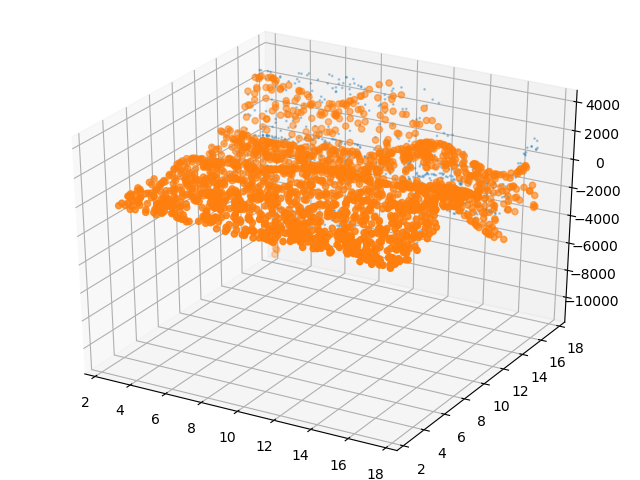
\includegraphics[width=\textwidth]{embedded_sinusoidal_small_perturbations_5d_to_2d_boring.png}
        \caption{Parabola Rembo}
        \label{fig:mouse}
    \end{subfigure}
    \caption{Top-Left: The 1D Parabola which is embedded in a 2D space.}\label{fig:animals}
\end{figure}

% SINUSOIDAL FUNCTION
\begin{figure}[H]
    \centering
    \begin{subfigure}[b]{0.3\textwidth}
        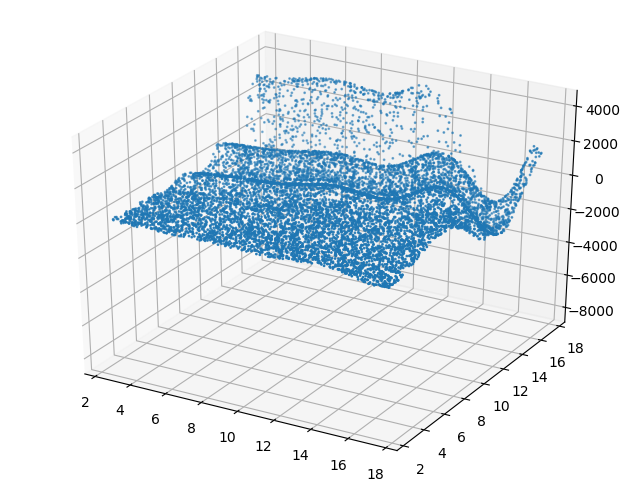
\includegraphics[width=\textwidth]{orig/embedded_sinusoidal_small_perturbations_5d_to_2d.png}
        \caption{Sinusoidal Original}
        \label{fig:gull}
    \end{subfigure}
    ~ %add desired spacing between images, e. g. ~, \quad, \qquad, \hfill etc. 
      %(or a blank line to force the subfigure onto a new line)
    \begin{subfigure}[b]{0.3\textwidth}
        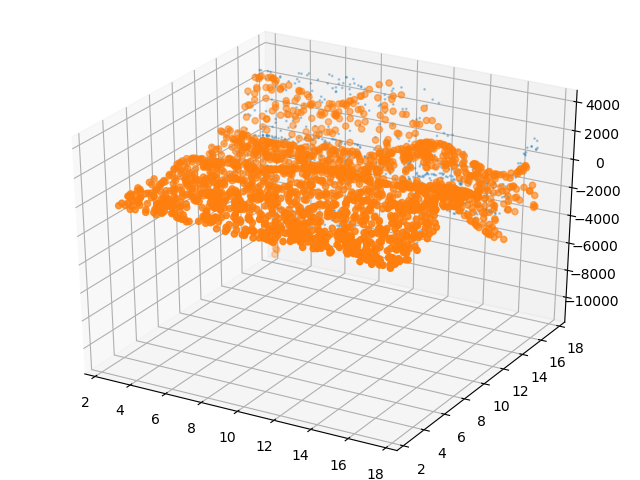
\includegraphics[width=\textwidth]{embedded_sinusoidal_small_perturbations_5d_to_2d_boring.png}
        \caption{Sinusoidal Boring}
        \label{fig:tiger}
    \end{subfigure}
        \vskip\baselineskip
 %add desired spacing between images, e. g. ~, \quad, \qquad, \hfill etc. 
    %(or a blank line to force the subfigure onto a new line)
    \begin{subfigure}[b]{0.3\textwidth}
        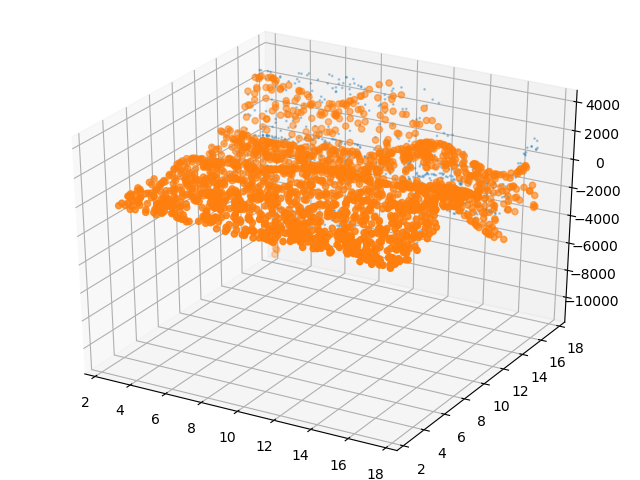
\includegraphics[width=\textwidth]{embedded_sinusoidal_small_perturbations_5d_to_2d_boring.png}
        \caption{Sinusoidal Tripathy}
        \label{fig:mouse}
    \end{subfigure}
        ~ %add desired spacing between images, e. g. ~, \quad, \qquad, \hfill etc. 
    %(or a blank line to force the subfigure onto a new line)
    \begin{subfigure}[b]{0.3\textwidth}
        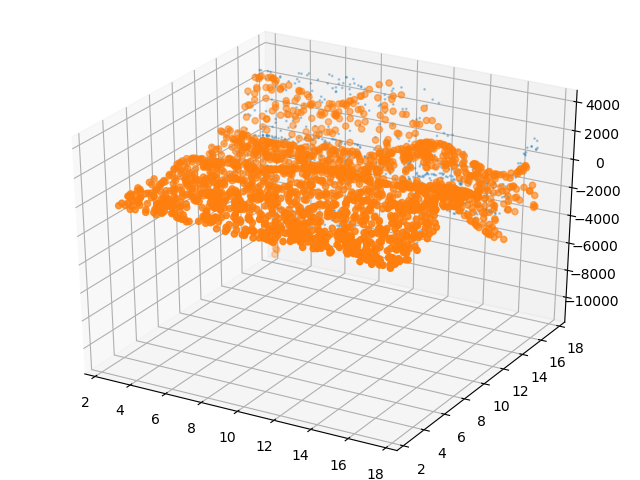
\includegraphics[width=\textwidth]{embedded_sinusoidal_small_perturbations_5d_to_2d_boring.png}
        \caption{Sinusoidal Rembo}
        \label{fig:mouse}
    \end{subfigure}
    \caption{Top-Left: The 2D Sinusoidal-Exponential Function which is embedded in a 5D space.}\label{fig:animals}
\end{figure}

% CAMELBACK FUNCTION
\begin{figure}[H]
    \centering
    \begin{subfigure}[b]{0.3\textwidth}
        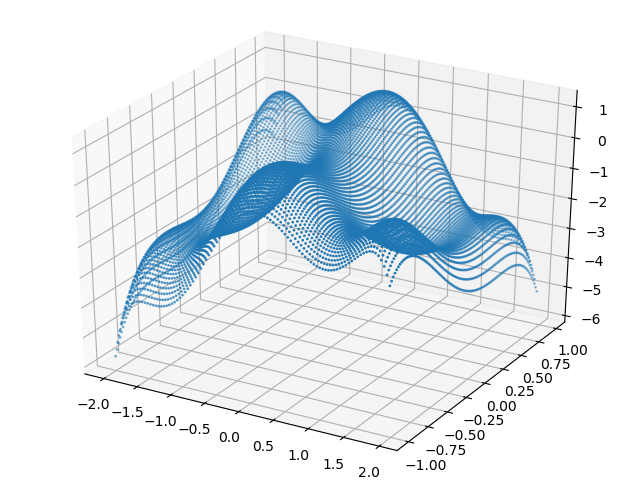
\includegraphics[width=\textwidth]{orig/embedded_camelback_5d_to_2d.png}
        \caption{Camelback Original}
        \label{fig:gull}
    \end{subfigure}
    ~ %add desired spacing between images, e. g. ~, \quad, \qquad, \hfill etc. 
      %(or a blank line to force the subfigure onto a new line)
    \begin{subfigure}[b]{0.3\textwidth}
        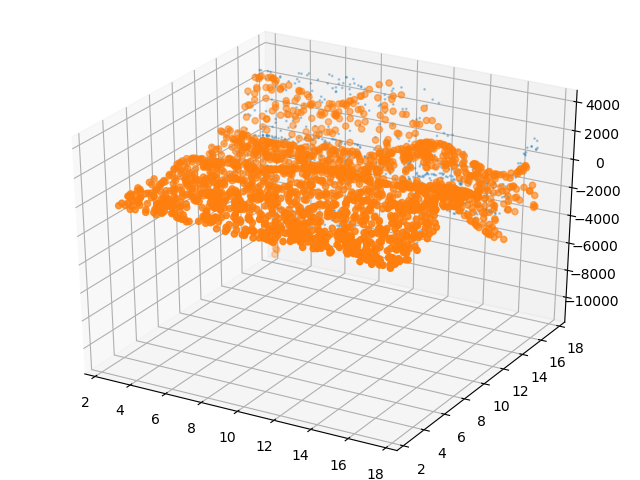
\includegraphics[width=\textwidth]{embedded_sinusoidal_small_perturbations_5d_to_2d_boring.png}
        \caption{Camelback Boring}
        \label{fig:tiger}
    \end{subfigure}
        \vskip\baselineskip
 %add desired spacing between images, e. g. ~, \quad, \qquad, \hfill etc. 
    %(or a blank line to force the subfigure onto a new line)
    \begin{subfigure}[b]{0.3\textwidth}
        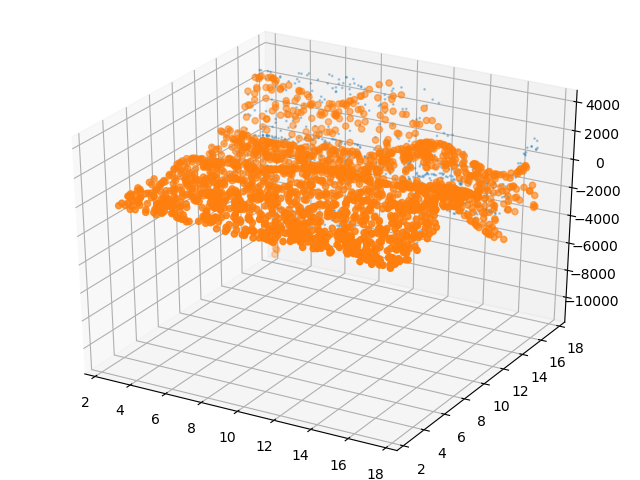
\includegraphics[width=\textwidth]{embedded_sinusoidal_small_perturbations_5d_to_2d_boring.png}
        \caption{Camelback Tripathy}
        \label{fig:mouse}
    \end{subfigure}
        ~ %add desired spacing between images, e. g. ~, \quad, \qquad, \hfill etc. 
    %(or a blank line to force the subfigure onto a new line)
    \begin{subfigure}[b]{0.3\textwidth}
        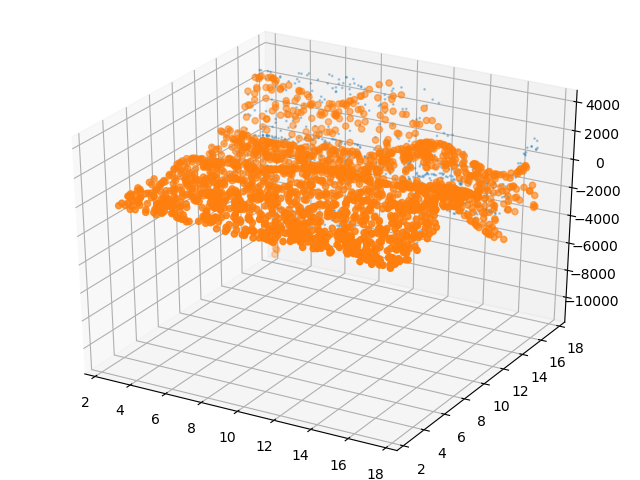
\includegraphics[width=\textwidth]{embedded_sinusoidal_small_perturbations_5d_to_2d_boring.png}
        \caption{Camelback Rembo}
        \label{fig:mouse}
    \end{subfigure}
    \caption{Top-Left: The 2D Camelback Function which is embedded in a 5D space.}\label{fig:animals}
\end{figure}

% ROSENBROCK FUNCTION
\begin{figure}[H]
    \centering
    \begin{subfigure}[b]{0.3\textwidth}
        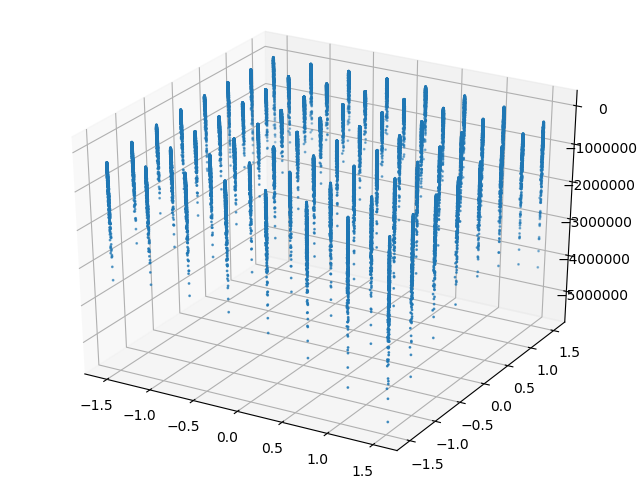
\includegraphics[width=\textwidth]{orig/embedded_rosenbrock_10d_to_5d.png}
        \caption{Rosenbrock Original}
        \label{fig:gull}
    \end{subfigure}
    ~ %add desired spacing between images, e. g. ~, \quad, \qquad, \hfill etc. 
      %(or a blank line to force the subfigure onto a new line)
    \begin{subfigure}[b]{0.3\textwidth}
        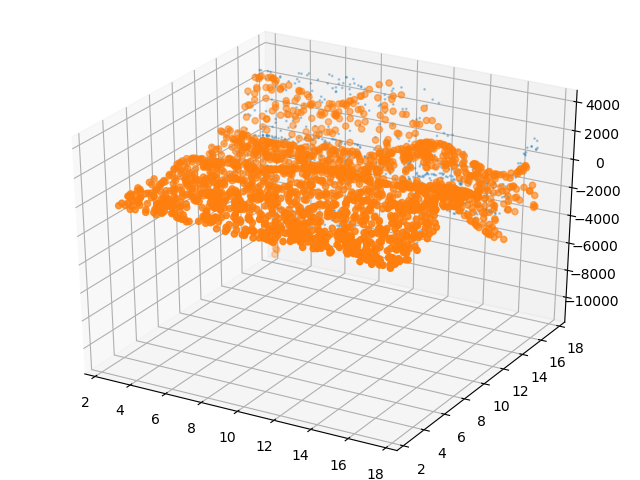
\includegraphics[width=\textwidth]{embedded_sinusoidal_small_perturbations_5d_to_2d_boring.png}
        \caption{Rosenbrock Boring}
        \label{fig:tiger}
    \end{subfigure}
        \vskip\baselineskip
 %add desired spacing between images, e. g. ~, \quad, \qquad, \hfill etc. 
    %(or a blank line to force the subfigure onto a new line)
    \begin{subfigure}[b]{0.3\textwidth}
        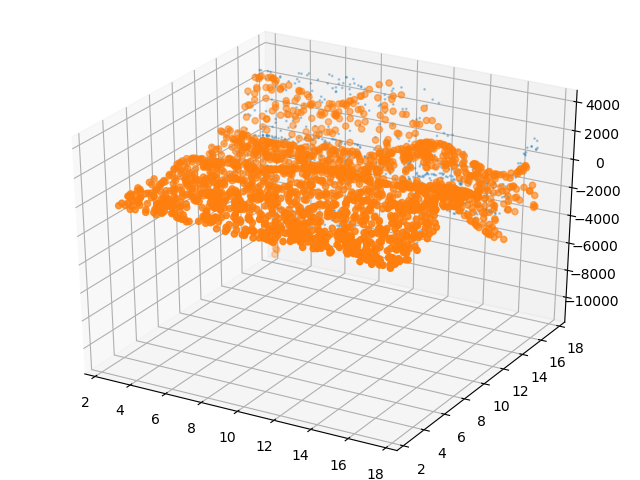
\includegraphics[width=\textwidth]{embedded_sinusoidal_small_perturbations_5d_to_2d_boring.png}
        \caption{Rosenbrock Tripathy}
        \label{fig:mouse}
    \end{subfigure}
        ~ %add desired spacing between images, e. g. ~, \quad, \qquad, \hfill etc. 
    %(or a blank line to force the subfigure onto a new line)
    \begin{subfigure}[b]{0.3\textwidth}
        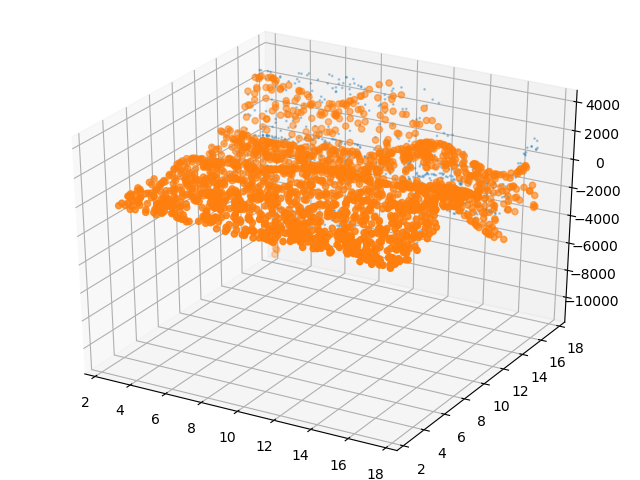
\includegraphics[width=\textwidth]{embedded_sinusoidal_small_perturbations_5d_to_2d_boring.png}
        \caption{Rosenbrock Rembo}
        \label{fig:mouse}
    \end{subfigure}
    \caption{Top-Left: The 5D Rosenbrock-Exponential Function which is embedded in a 10D space. We visualize the function using the first two principal components (projection using PCA)}\label{fig:animals}
\end{figure}

